\chapter{Implementation}

\section{Assembly and dependency structure}

The function \code{app.NewRouter} receives a set of ready-made services and returns the complete HTTP handler: public routes, the JSON API under \code{/api} and the web interface. The production entry point \code{cmd/api} builds the services on PostgreSQL repositories; the tests build the same services on in-memory repositories or on a real database and call the same function. As a result no test uses a hand-written approximation of the router, and a route that is missing in production is missing in the tests as well.

The server reads its configuration from environment variables (Table~\ref{tab:config}). The first administrator is created at start-up from \code{ADMIN\_EMAIL} and \code{ADMIN\_PASSWORD} if no such account exists, which replaces the removed public registration.

\begin{table}[H]
\centering
\caption{Main configuration variables}
\label{tab:config}
\small
\begin{tabularx}{\textwidth}{@{}lX@{}}
\toprule
Variable & Meaning \\
\midrule
\code{DATABASE\_URL} & PostgreSQL connection string \\
\code{JWT\_SECRET} & Signing key for sessions; must be changed in production \\
\code{PORT} & HTTP port (8080 by default) \\
\code{ADMIN\_EMAIL}, \code{ADMIN\_PASSWORD} & Bootstrap administrator \\
\code{COOKIE\_SECURE} & \code{true} when served over HTTPS \\
\code{LOGIN\_RATE\_LIMIT} & Login attempts per minute per address (10 by default) \\
\code{REMINDER\_HOUR} & Hour of the attendance reminder; $-1$ disables it \\
\code{SMTP\_*}, \code{EMAIL\_LOG} & E-mail delivery, or log-only mode for demonstrations \\
\bottomrule
\end{tabularx}
\end{table}

\section{Five-point marks}
\label{sec:fivepoint}

The change from 0--100 scores to marks from 1 to 5 touches four layers, and each layer has its own check.

\textbf{Service.} Validation is a single function that rejects anything that is not a whole number in range, including NaN. The final mark of a subject is computed by one function used by every report (Listing~\ref{lst:marks}). The request type keeps the mark as a floating-point number so that a client sending \code{3.5} receives a clear message instead of a decoding error.

\begin{lstlisting}[caption={Validation and final mark (simplified from \code{grade\_service.go})},label={lst:marks},float=htbp]
const (MinMark = 1; MaxMark = 5)

func validateMarks(m float64) error {
    if math.IsNaN(m) || m != math.Trunc(m) || m < MinMark || m > MaxMark {
        return fmt.Errorf("mark must be a whole number from %d to %d", MinMark, MaxMark)
    }
    return nil
}

func FinalMark(avg float64) int {
    if avg <= 0 { return 0 }                // no marks
    f := int(math.Floor(avg + 0.5))         // half rounds up: 4.5 -> 5
    return min(MaxMark, max(MinMark, f))
}
\end{lstlisting}

\textbf{Database.} Migration 000003 first converts existing scores with the bands of Table~\ref{tab:conversion}, then replaces the old range constraint by \code{chk\_grades\_five\_point}, which accepts only 1, 2, 3, 4 and 5. The order matters: adding the constraint first would fail on legacy rows. The down migration removes the new constraint, maps each mark to the middle of its band and restores the old one.

\textbf{Reports.} A report contains the individual marks, one row per subject with the average, the final mark and the number of marks, and the overall average (Section~\ref{sec:final}). The earlier grade-point and credit-weighted fields were removed from the API, so a client that still reads them fails visibly instead of showing stale semantics.

\textbf{Permissions.} Any administrator or teacher with access to the class may give a mark; only an administrator or the teacher who recorded a mark may change or delete it. Recording a mark creates a notification for the pupil and the linked parents.

\textbf{Interface.} In the gradebook (Figure~\ref{fig:gradebook}) the teacher chooses a class, a subject and a term and sees one row per pupil with the marks in date order, the average and five coloured buttons labelled 5 to 1. Pressing a button gives that mark immediately; clicking an existing mark opens it for change or removal. The five-point scale is repeated as a legend on the pupil's marks page and on the home page.

\begin{figure}[H]
\centering
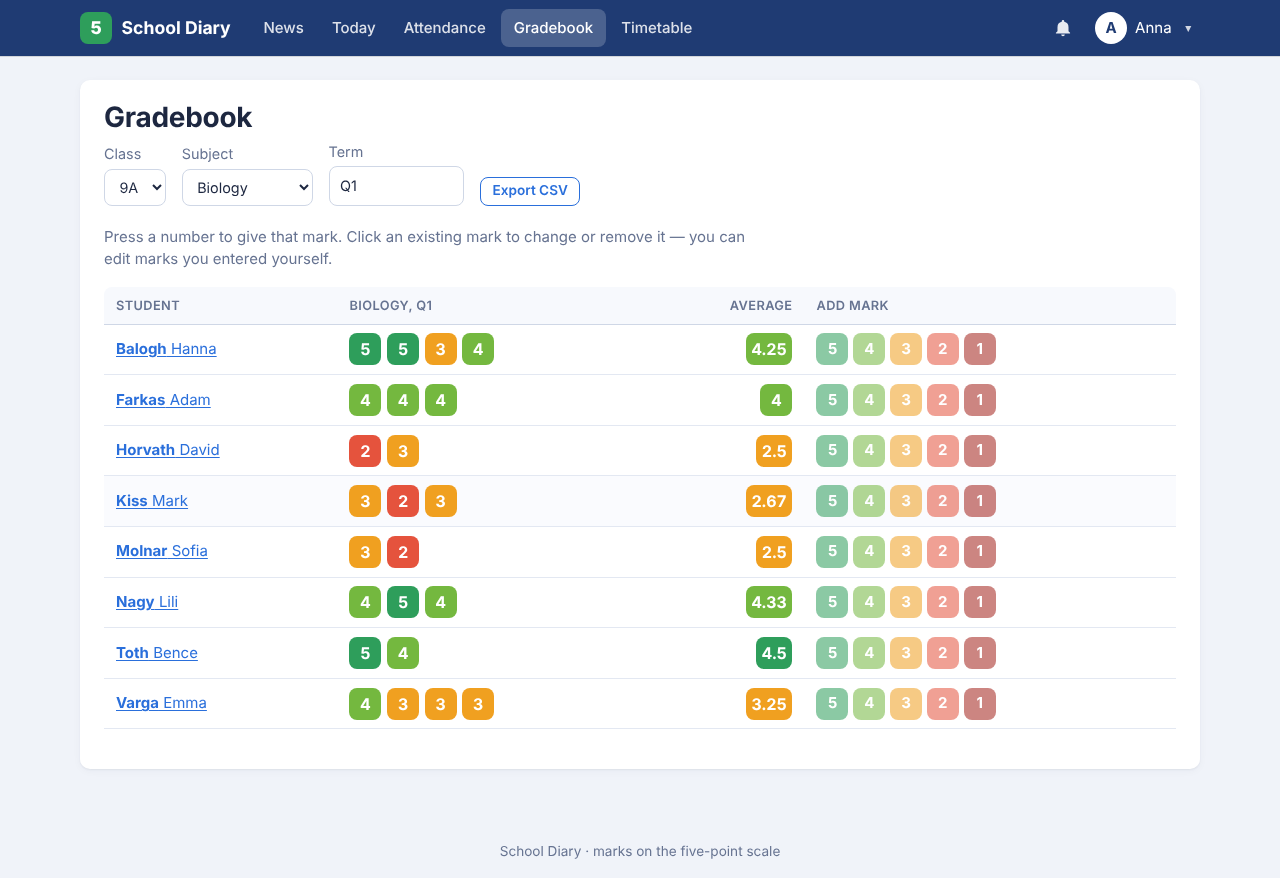
\includegraphics[width=0.92\textwidth]{fig/gradebook.png}
\caption{Teacher's gradebook: marks by pupil with averages and one-press mark entry}
\label{fig:gradebook}
\end{figure}

\section{Attendance and timetable rules}

Attendance is recorded in bulk for a class and a day; recording again for the same day overwrites the previous status, which matches the way a teacher corrects a sheet. The percentage follows Equation~(3). The low-attendance check compares the percentage before and after the record and fires only when it crosses the 75\,\% threshold with at least five recorded days.

The timetable rejects three kinds of conflict: two lessons of the same class, of the same teacher or in the same room whose time intervals overlap on the same weekday. Intervals are treated as half-open, so a lesson ending at 09:40 and another starting at 09:40 do not conflict. A lesson is also rejected if the teacher has not been qualified to teach the subject. The conflict test is a pure function over the lessons of one day, which makes it easy to test exhaustively.

\section{School news and the home page}

The new home page required a change in routing. The root path \code{/} became public and shows the news feed; the role-specific start page ``Today'' moved to \code{/dashboard}, and a successful login redirects there. A signed-in user sees the same home page inside the normal menu, a guest sees a sign-in button and a short explanation (Figure~\ref{fig:home}).

\begin{figure}[H]
\centering

\includegraphics[width=0.92\textwidth]{fig/home.png}
\caption{Public home page with the school news feed and the five-point legend}
\label{fig:home}
\end{figure}

News items live in the table \code{news} with a title (up to 200 characters), a text (up to 10\,000 characters), a pinned flag, an author and timestamps. The feed is ordered by pinned flag and then newest first, which is exactly what the index \code{idx\_news\_feed} supports. The JSON API exposes \code{GET /api/news} publicly and \code{POST}, \code{PUT} and \code{DELETE} to administrators only; the service rejects anyone else with 403 even if a handler were misconfigured.

The text is plain text. The page splits it into paragraphs at blank lines and escapes each paragraph, so markup typed by an administrator is shown literally. A feed card shows the beginning of the text collapsed into one line and shortened to about 260 characters at a word boundary. An earlier version showed only the first paragraph, which made a news item that begins with a greeting look empty; the final version joins the paragraphs, and a unit test covers this case. Administrators manage news on a separate page (Figure~\ref{fig:adminnews}) with a form for a new item and a table of published items with edit and delete actions.

\begin{figure}[H]
\centering
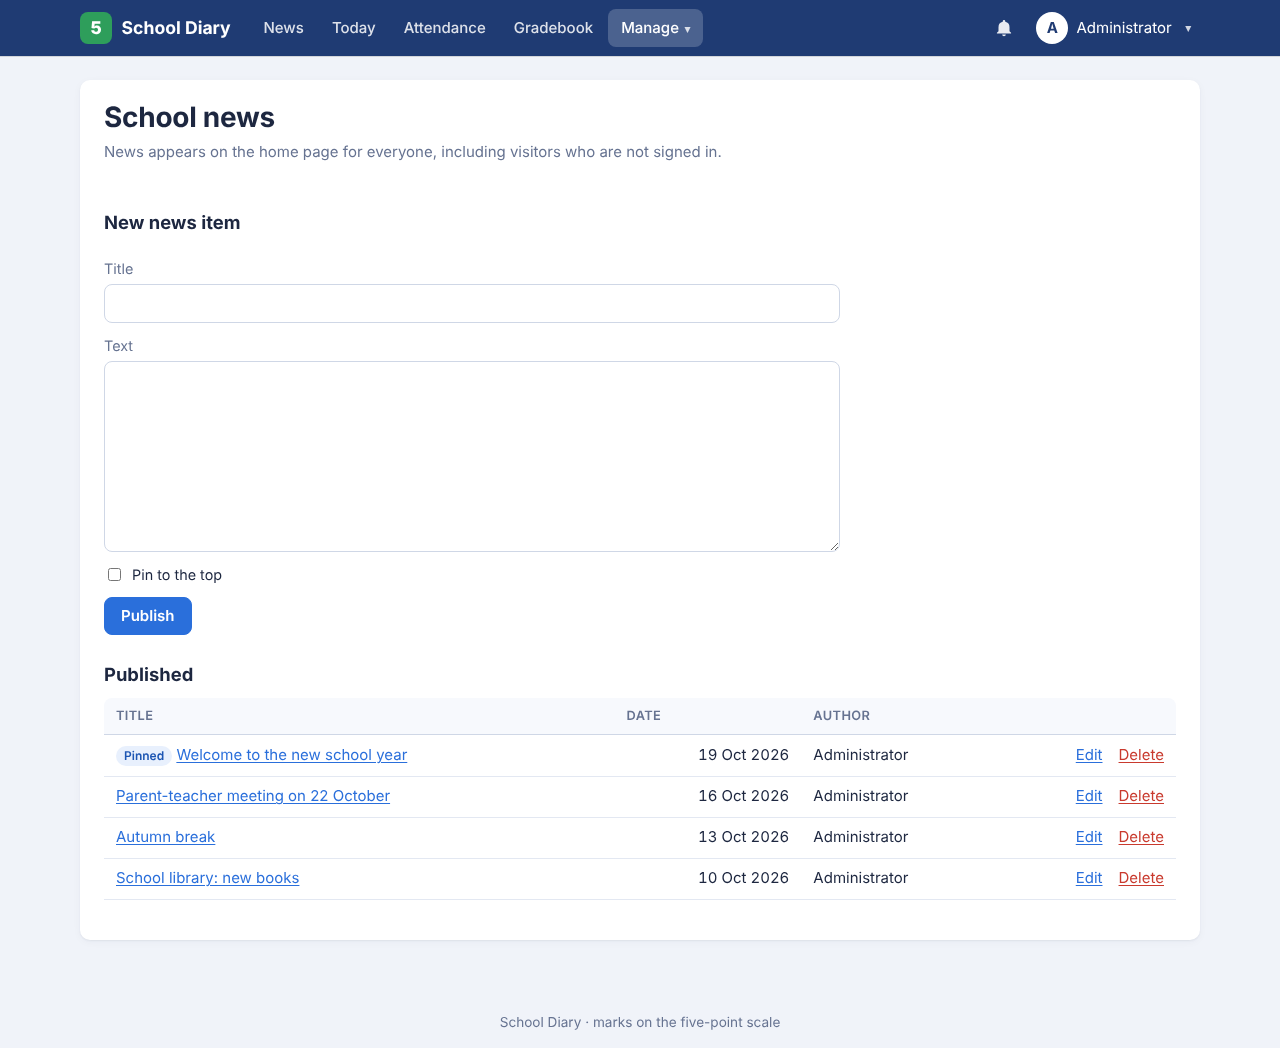
\includegraphics[width=0.92\textwidth]{fig/admin_news.png}
\caption{Administrator's news page: publish form and list of published items}
\label{fig:adminnews}
\end{figure}

\section{The diary interface}

The interface replaces the earlier side-bar layout with a top bar and white cards on a light background. The menu depends on the role: pupils see News, Today, Diary, Marks, Attendance and Timetable; teachers see Attendance and Gradebook; administrators additionally have a Manage menu. A bell with an unread counter links to the notifications.

The central page is the weekly diary (Figure~\ref{fig:diary}). The function that builds it takes the Monday of the requested week, the pupil's class timetable and the pupil's marks and returns one block per weekday. Saturday and Sunday appear only when they contain lessons or marks. A mark is placed beside the \emph{first lesson of its subject on the day the mark was given}; marks for which no lesson exists that day are listed under ``Other marks'' in the same card, so no mark is ever hidden. Today is highlighted, and the buttons ``Previous'', ``This week'' and ``Next'' move through weeks through a query parameter, which also makes a particular week bookmarkable. Parents reach the same view for each child.

\begin{figure}[H]
\centering
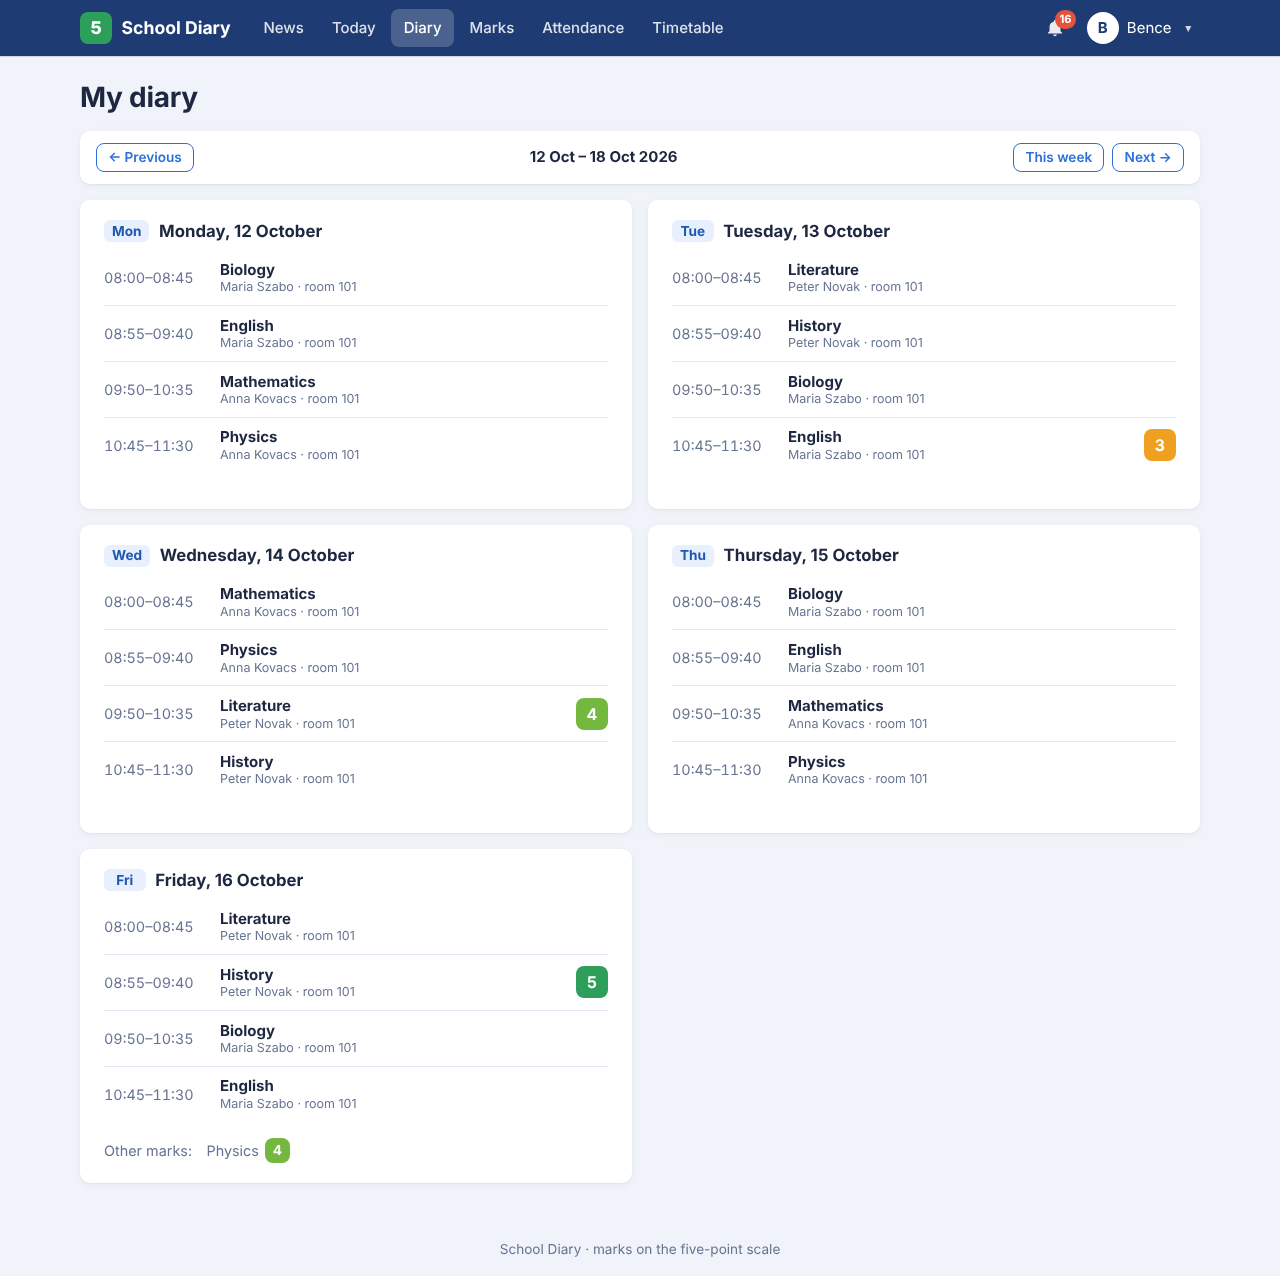
\includegraphics[width=0.92\textwidth]{fig/diary.png}
\caption{Weekly diary of a pupil: lessons by day with the marks received}
\label{fig:diary}
\end{figure}

The marks page (Figure~\ref{fig:marks}) shows the overall average, the number of marks and subjects, and for each subject all marks in date order, the average and the final mark. A caption explains that the final mark is the average rounded half up.

\begin{figure}[H]
\centering
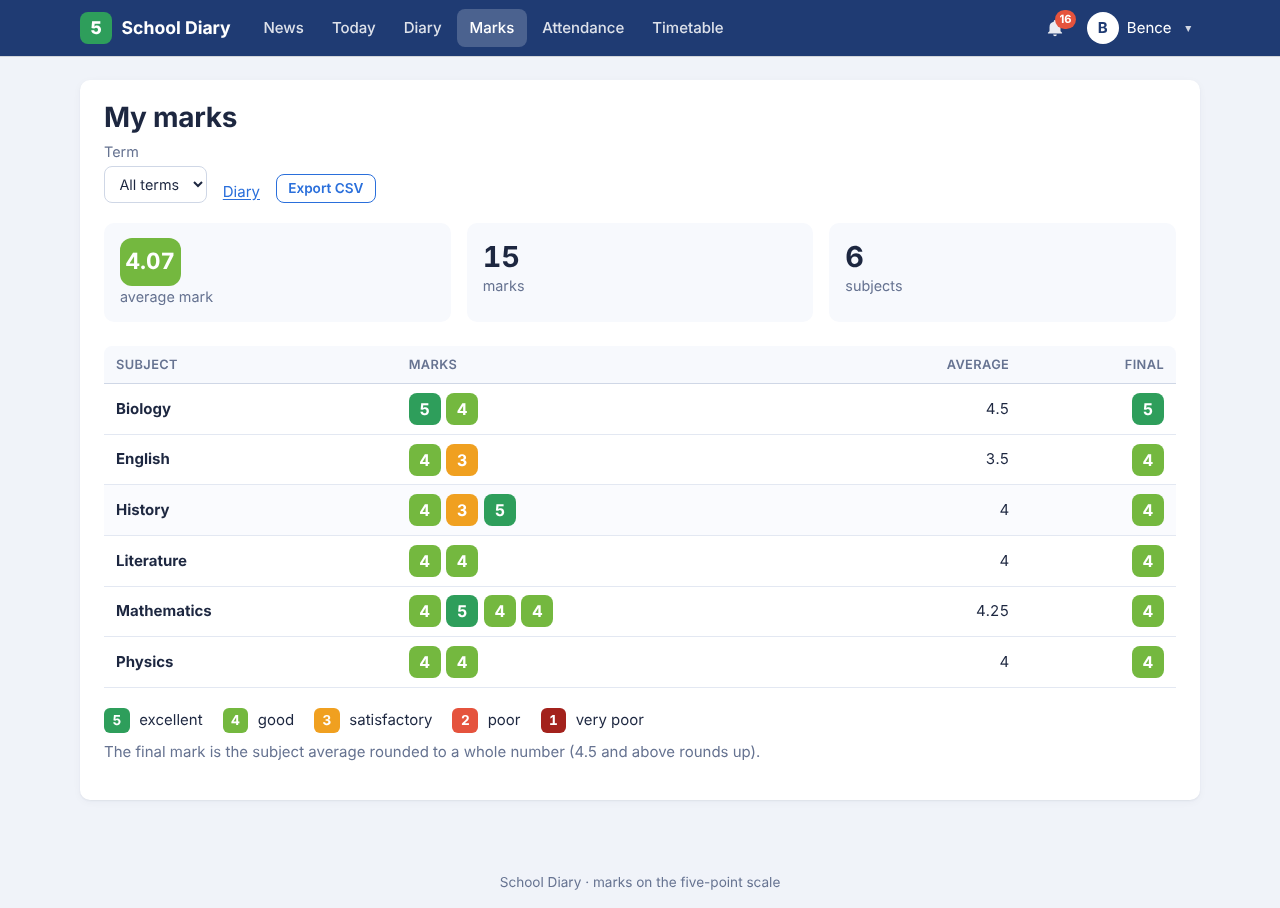
\includegraphics[width=0.92\textwidth]{fig/marks.png}
\caption{A pupil's marks by subject with averages and final marks}
\label{fig:marks}
\end{figure}

Responsive behaviour is achieved with CSS grid and wrapping flex rows. On a viewport 390\,px wide the home page does not scroll horizontally (Section~\ref{sec:ui}). Interface text is English; all strings are in templates, which keeps a later translation mechanical.

\section{Reports, export and demonstration data}

Marks and attendance can be exported as CSV for a pupil and for a whole class. The writer starts the file with a UTF-8 byte-order mark so that spreadsheet programs detect the encoding, and prefixes any cell that begins with \code{=}, \code{+}, \code{-}, \code{@}, a tab or a carriage return with an apostrophe so that it cannot be executed as a formula \cite{owaspcsv}. The export service reuses the report functions, which keeps the exported averages identical to the screen.

The command \code{cmd/seed} loads a demonstration school into an empty database: an administrator, teachers, two classes (9A and 9B) with 16 pupils in total, parents, subjects, a weekly timetable, marks from 2 to 5 spread over the last school days, attendance and four news items. It exercises every repository against real SQL and gives every role an account to try.
